\documentclass[tikz, border=2mm, preview]{standalone}
\usepackage{xcolor}
\definecolor{customBlue}{RGB}{11, 61, 98}%
\usetikzlibrary{3d}

\begin{document}
    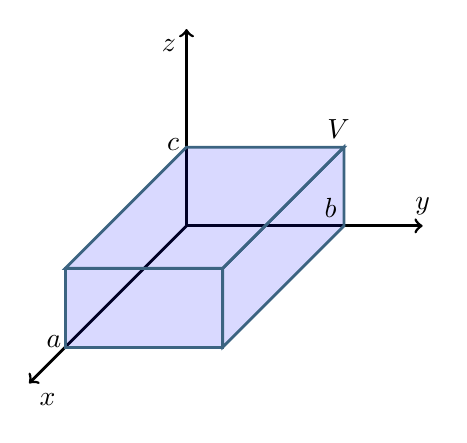
\begin{tikzpicture}
        % Ejes
        \begin{scope}[->, canvas is plane]
            \draw[line width = 1pt] (0,0,0) -- (xyz spherical cs:radius=2.5) node[below left] {$z$};
            \draw[line width = 1pt] (0,0,0) -- (xyz spherical cs:radius=4,latitude=45, longitude=-135) node[below right] {$x$};
            \draw[line width = 1pt] (0,0,0) -- (xyz spherical cs:radius=3,longitude=90) node[above] {$y$};
        \end{scope}
        % Paralelepípedo
        \begin{scope}[canvas is xz plane at y=1]
            \draw[color=customBlue!80, line width=1pt, fill=blue, fill opacity=0.15] (0, 0) -- (2, 0) -- (2, 4) -- (0, 4) -- cycle;
        \end{scope}
        \begin{scope}[canvas is yz plane at x=2]
            \draw[color=customBlue!80, line width=1pt, fill=blue, fill opacity=0.15] (0, 0) -- (0, 4) -- (1, 4) -- (1, 0) -- cycle;
        \end{scope}
        \begin{scope}[canvas is xy plane at z=4]
            \draw[color=customBlue!80, line width=1pt, fill=blue, fill opacity=0.15] (0, 0) -- (2, 0) -- (2, 1) -- (0, 1) -- cycle;
        \end{scope}
        % Cargas
        \node at (2.7, 2, 2) {\(V\)};
        \node at (0.8, 1.02, 6.45) {\(a\)};
        \node at (2.6, 1, 2) {\(b\)};
        \node at (0.6, 1.8, 2) {\(c\)};
    \end{tikzpicture}
\end{document}
